\section{Architectural Comparison}
\label{sec:architectural_comparison}

\subsection{Isotropic columnar vs. hierarchical multi-stage architectures}
Comparing ResMLP and RepMLP highlights two different design choices in modern Vision MLPs:

\begin{table}[h]
\centering
\adjustbox{max width=\linewidth}{%
\begin{tabularx}{\linewidth}{lXX}
\toprule
\rowcolor{aivnGreen!12}
\textbf{Dimension} & \textbf{ResMLP}~\cite{touvron2021resmlp} & \textbf{RepMLP}~\cite{ding2022repmlp} \\
\midrule
\textbf{Macro topology} & Isotropic columnar (uniform $D=256$, $N=64$ throughout) & Hierarchical multi-stage ($16*16 \to 8*8 \to 4*4$) \\
\textbf{Downsampling} & Single patch embedding ($P=4$ at stem) & Multi-step downsampling ($P=2$ plus transitions) \\
\textbf{Spatial mixing} & Global linear matrix $\mathbf{W}_{\text{token}} \in \mathbb{R}^{N \times N}$ & Partition-based FC3 with local sharesets $S$ \\
\textbf{Locality injection} & None (pure linear token projection) & Multi-branch depthwise convolutions ($3*3, 1*1$) \\
\textbf{Channel mixing} & Affine scaling + 2-layer FFN (GELU) & Global perceptron (SE attention) + 2-layer FFN \\
\textbf{Inference graph} & Identical to training graph & Merged via structural re-parameterization \\
\bottomrule
\end{tabularx}%
}
\vspace{0.6em}
\caption{Structural and operational comparison between ResMLP and RepMLP baselines.}
\label{tab:arch_comparison}
\end{table}

\begin{figure}[t]
\centering
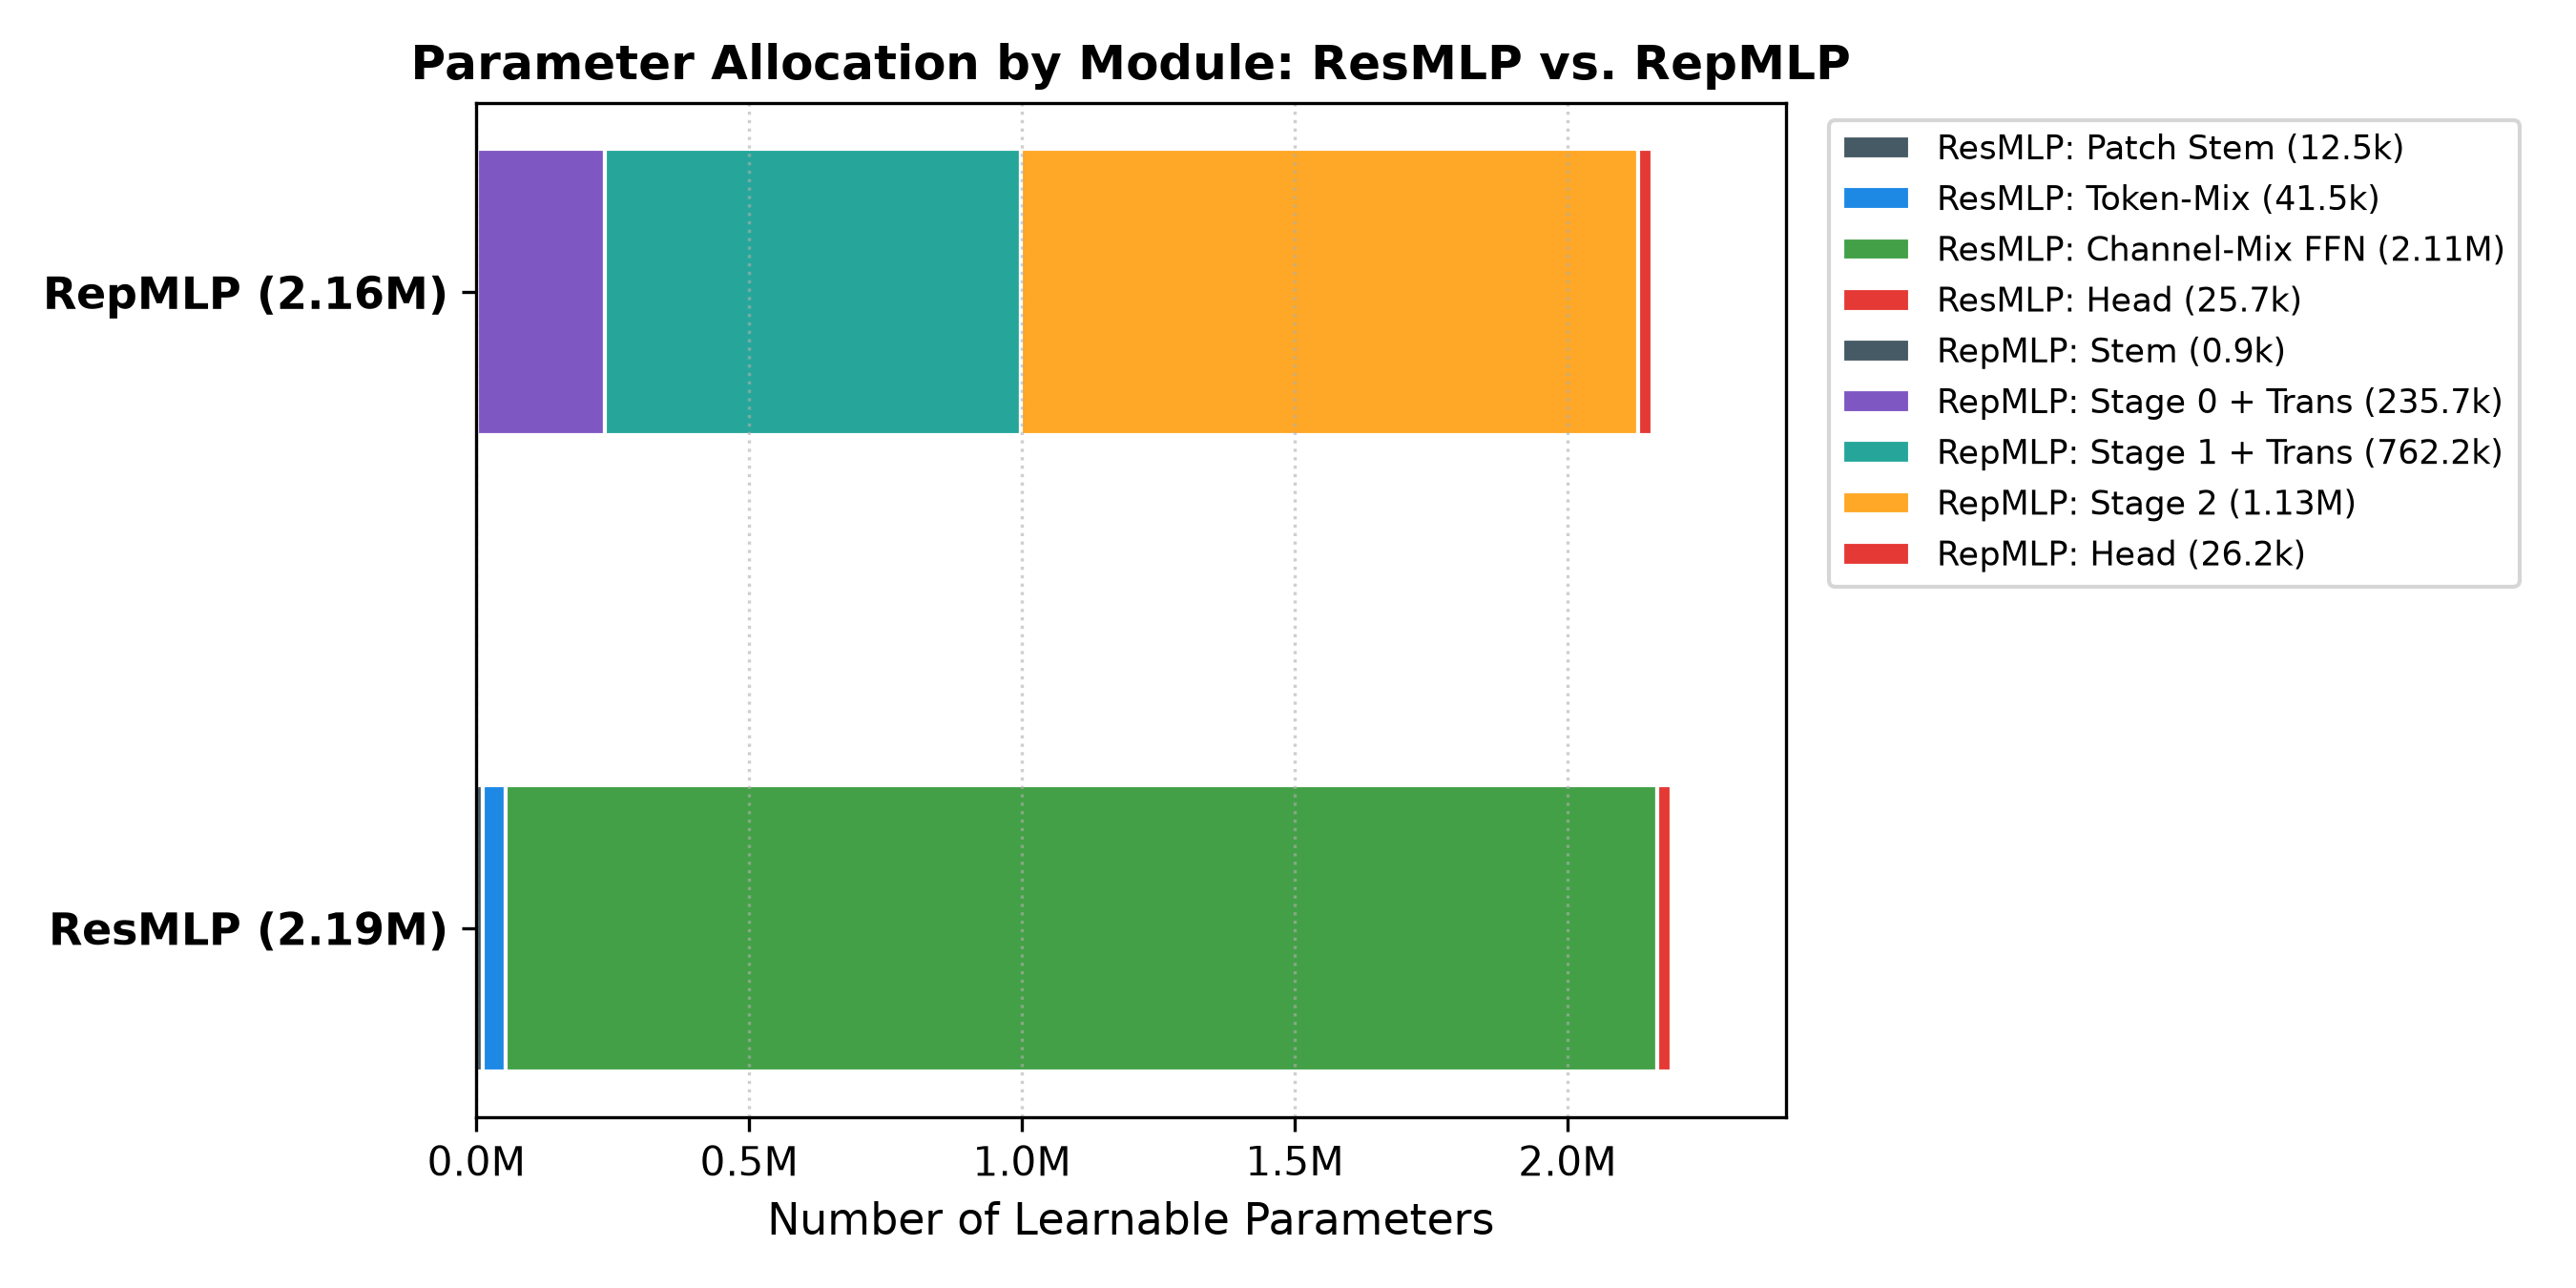
\includegraphics[width=0.75\textwidth]{figures/param_breakdown.png}
\caption{Parameter breakdown: ResMLP concentrates $96.36\%$ of its parameters in channel FFNs, while RepMLP spreads capacity across hierarchical stages and multi-scale units.}
\label{fig:param_breakdown}
\end{figure}

\subsection{How spatial tokens interact}
The main difference between the two models is how they handle spatial relationships between image patches:
\begin{itemize}[leftmargin=1.5em]
    \item \textbf{ResMLP global linear mapping:} For patch sequence $\mathbf{Z} \in \mathbb{R}^{B \times N \times D}$, the token-mixing sublayer computes:
    \begin{equation}
        \mathbf{Y}_{\text{spatial}} = \text{Affine}_2 \left( \left( \text{Affine}_1(\mathbf{Z})^{\top} \mathbf{W}_{\text{token}} + \bm{b}_{\text{token}} \right)^{\top} \right) + \mathbf{Z}.
    \end{equation}
    Because $\mathbf{W}_{\text{token}}$ connects every patch to every other patch, it covers the whole image in one step. However, it does not know which patches are nearby: neighboring patches are treated just like patches on opposite corners of the image.
    
    \item \textbf{RepMLP partitioned communication:} RepMLP addresses this by dividing the feature map into small local patches ($h * w$) and training them alongside depthwise conv branches. While this brings strong locality, it requires reshaping and slicing tensors back and forth, which makes the model more complex than a standard MLP.
\end{itemize}

\subsection{Linear additivity and re-parameterization}
From replicating both models, we arrive at an important design insight:
\begin{equation}
    \text{Linear additivity principle:} \quad \mathcal{T}_{\text{fused}}(\mathbf{x}) = \mathbf{W}_{\text{linear}} \mathbf{x} + \text{Conv}(\mathbf{x}) = \left(\mathbf{W}_{\text{linear}} + \mathbf{W}_{\text{conv}}\right) \mathbf{x} + \bm{b}_{\text{conv}}.
\end{equation}
In models like MLP-Mixer, token mixing uses two linear layers with an activation in between: $\mathbf{Z}_{\text{out}} = \sigma(\mathbf{Z} \mathbf{W}_1) \mathbf{W}_2$. Because of the non-linear activation $\sigma$, we cannot add a parallel convolution branch and fold it into the weights at test time.

In ResMLP, however, Touvron et al.~\cite{touvron2021resmlp} showed that token mixing can work well using a \textbf{purely linear layer} $\mathbf{W}_{\text{token}} \in \mathbb{R}^{N \times N}$, with non-linearities placed only in the channel-mixing FFN. 

This makes ResMLP an ideal fit for structural re-parameterization: because token mixing is purely linear, we can add parallel depthwise conv branches during training, and fold them into the single linear matrix at test time without any extra runtime cost.
